% !TeX document-id = {612e9a85-cc42-4184-aff3-32683cbba82e}
% !TeX TXS-program:compile = txs:///pdflatex/[--shell-escape]
%
% You may wish to use some of the following options of the iitthesis
% package:
%
% fullpageDraft      avoid the margins necessary for proper binding and
%   just view or print a draft.
% beforeExam         makes the personal acknowledgements invisible; use
%   this to print the copies you submit initially to the grad school
%   for sending to the examiners (who shouldn't see these). For the
%   final submission, drop this option.
% noabbrevs          no notation & abbreviations list will be included
%   in the thesis.
%
% Additionally, you must specify the degree for which you're writing
% your thesis (MSc/PhD/MArch etc.)
%
\documentclass[MSc,beforeExam, noabbrevs]{misc/iitthesis}


% Definitions of info fields for the thesis - subject, advisor,
% faculty, acknowledgements, etc. etc. This file must contain Hebrew
% text, so the question of its character set encoding is significant.
% This templated uses the iso-8859-8-i charset (i.e. single-byte logical 
% Hebrew; it's about the same as the windows-1255 codepage, but not the
% same as UTF-8) - and this works with MikTeX 2.9 and using pdfelatex.
% With your TeX distribution you might need to create files in the
% UTF-8 charset.
\authorEnglish{Oron Port}
%\authorHebrew{�� ���}

\titleEnglish{DFiant: A Dataflow Hardware Description Language}
%\titleHebrew{??? ?????????? ?????? ????? ????? ??? ???? ????-???? ?????}

\disciplineEnglish{Electrical Engineering}
%\disciplineHebrew{���� �����}

\supervisionEnglish{This research was carried out under the supervision of Prof.~Yoav Etsion, in the Faculty of Electrical Engineering.}
\supervisionHebrew{����� ���� �������� �� ������� ������� ������, ������� ����� �����.}

\GregorianDateEnglish{April 2017}
% In Hebrew-language text with babel, if you use a number, the digit order
% gets reversed; if you \L{123} it, you get the number in the English-language
% font glyphs for numbers. Instead, use \beginL 123 \endL - which only changes
% the direction, not the language
\GregorianDateHebrew{����� \beginL 2012 \endL}
\JewishDateEnglish{Tishrei 5776}
\JewishDateHebrew{��� ����"�}

\financialAcknowledgementEnglish{}
%\financialAcknowledgementHebrew{���� ���� ����� ������� �� ����� ���� ��.}

\publicationInfoEnglish{%
}

\publicationInfoHebrew{%
)�������� ��������, ������� ����, ���� ������ ��� ����� ���"� ������� �������; ����� ��� ����� �� ����� ��� ���������... ���� �� ����� ����� \L{\texttt{thesis-fields.tex}}. �� ����� ����� ���� ���� �� ����� ��� �� ������ ������ �� ������� ��� ����� �����.(
��� �� ������� ������ �� ������ ������� ��� ����� ������� ����� ������ ������-�� ����� ����� ���� �������� �� �����, ��� ��������� �������� ����� ����:%

\begin{otherlanguage}{english}%
% No need to mention the bibliography file this time, as it has already been used in
% the English invocation
\butcheredbibliography{pubinfo}{front/pubinfo}
\end{otherlanguage}%
}

\thesisbibfiles{back/general}
\thesisbibstyle{alpha}


% Personal acknowledgements (are only used for the post-exam
% version)
\personalAcknowledgementEnglish{
(Note that these acknowledgement only appear in the copy printed after the exam:) I would like to thank my advisor, my parents, my friends, etc. etc.

Add any thank-yous, acknowledgements, personal comments you wish to make here (in \texttt{personal-acks.tex}).
}

\personalAcknowledgementHebrew{
)���/� ��: ����� ��� ������� �� ����� ������ ���� ������, ��� �����.(
��� ���� ������ ����� ���, ������, ������, ���' ���'.

���� ������ ��� ����� ������ ������ ���.
}


% The abstract in Hebrew and in English should have its own file.
%
% Notes:
% - You can split this one, and have separate files for the English
%   and the Hebrew abstract
% - regulations require the English abstract contain between 200 and
%   500 words, and the Hebrew abstract contain between 1,000 and 2,000
%   words (making it something between an abstract and an introduction
%   with an overview of results).
% - Be careful with links in Hebrew text (wrap them in \L{}).
% As a general rule, do not put math, special symbols or citations
% in the abstract
\begin{abstract}
Today's dominant hardware description languages (HDLs), namely Verilog and VHDL, rely on limited register-transfer-level (RTL) constructs. These constructs tightly couple design functionality with timing requirements and target-device constraints. As hardware designs and device architectures become increasingly more complex, these dominant HDLs yield verbose and unportable code.
To raise the level of abstraction, several high-level synthesis (HLS) tools were introduced, usually based on software languages such as C. Unfortunately, designing hardware with sequential software language semantics comes at a price; the designer loses the ability to control hardware construction and data scheduling, which is crucial in many design use-cases. 

In this paper we further extend DFiant, a Scala-based HDL that uses the dataflow model to decouple functionality from implementation constraints.
DFiant's frontend enables functional bit-accurate hardware description, while maintaining a complete timing-agnostic and device-agnostic code. DFiant bridges the gap between software programming and hardware construction, driving an intuitive functional object oriented code into a high-performance hardware implementation.

For a proof of concept, we implemented a compiler frontend for DFiant, which transforms DFiant code into a dataflow graph, and a preliminary auto-pipelining backend, which maps the graph into synthesizable Verilog code. We further implemented two test cases in DFiant: an Advanced Encryption Standard cipher block and an IEEE-754 floating point multiplier. We compared both test cases against modern design flows. Our results demonstrate that DFiant can greatly simplify hardware designs yet still maintain competitive performance.
\end{abstract}

%We defined a new language from the ground up, borrowing concepts from hardware, dataflow and software languages. The result is a strongly-typed, purely synthesizable extendable language frontend, fit for both general-purpose and high level hardware description.


% Just write down your abstract here, no special commands necessary except for the \abbreviationsAndNotation{
% before this text is used and a closing } at the end of it

\abbreviationsAndNotation{
\begin{tabular}{p{2cm}@{:\quad}l}
AES & advanced encryption standard \\
CAFEO & Constructible for Any FPGA, Expressed Once \\
CDC & clock domain crossing \\
DF & dataflow \\
DFG & dataflow graph \\
DSP & digital signal processor \\
EDA & electronic design automation \\
FIFO & first in first out \\
FP & floating-point \\
FPGA & field-programmable gate array \\
FW & future work \\
HDL & hardware description language \\
HLS & high-level synthesis \\
IP & intellectual property \\
LUT & look-up table \\
N/A & not applicable \\
PD & propagation delay \\
RTL & register-transfer level \\
SoC & system on chip \\
\end{tabular}
}


% Additional machinery relevant to any thesis
% (it's not part of the document class because it's not absolutely
% necessary and not everyone might like it)
\usepackage{misc/iitthesis-extra}

% Definitions useful for anything you write, which you also
% include in any articles, presentations, HW assignments and other
% documents. May contains macros for notation algebra, logic,
% calculus and other fields, as well as general shorthands and
% LaTeX tricks, and package use commands
% General-purpose definitions and inclusions
% you are using in any document 
% (regardless of its class and style files used),
% e.g. package uses:

%\usepackage{xspace}

% and macros/command defintions:

%\newcommand{\complexityclass}[1]{{\bf #1}\xspace}
%\newcommand{\NPTIME}{\complexityclass{NP}}

% For this template, we'll only have one single command,
% necessary for including graphics...
\usepackage{graphicx}% http://ctan.org/pkg/graphicx

% leaving example code for floating figure outside of text
%  \makebox[\textwidth][c]{\includegraphics[width=1.2\textwidth]{graphics/Classes.eps}}%


% Definitions, settings and tweaks for this thesis specifically

% This file should contain your own definitions specific
% only to this thesis;

% What it contains below is used 
% simply for generating dummy text in the sample 
% content provided with the template (see mainchap1.tex);
% so you can safely delete this when creating your own
% thesis

\newcommand{\cf}{\textit{CAFEO}~}
\newcommand{\cfns}{\textit{CAFEO}}
\usepackage{color}
\newcommand{\Q}[1]{\textcolor{red}{[#1]}}
\usepackage{graphicx}
\usepackage{array}
\usepackage{fixltx2e}
\usepackage{amsmath}
\usepackage{amssymb}

\usepackage{minted} % Required to display colored code properly
%hack for minted to get rid of syntax error boxes
\makeatletter
\AtBeginEnvironment{minted}{\dontdofcolorbox}
\def\dontdofcolorbox{\renewcommand\fcolorbox[4][]{##4}}
\makeatother
\usepackage[utf8]{inputenc}
%\usepackage{tipa}
\usepackage[export]{adjustbox}
%\usepackage[ampersand]{easylist}
\raggedbottom
%\setlength{\belowcaptionskip}{-10pt}
\usepackage{pdfpages}
\usepackage{afterpage}
\newcommand\blankpage{%
    \null
    \thispagestyle{empty}%
    \addtocounter{page}{-1}%
    \newpage}
    
\usepackage{xpatch}
\xpatchcmd{\algorithmic}{\setcounter}{\algorithmicfont\setcounter}{}{}
\providecommand{\algorithmicfont}{}
\providecommand{\setalgorithmicfont}[1]{\renewcommand{\algorithmicfont}{#1}}
\renewcommand{\algorithmiccomment}[1]{{\tiny\hfill$\triangleright$ #1}}
\newcommand{\INDSTATE}[1][1]{\STATE\hspace{#1\algorithmicindent}}

% *** NON FLOAT MINIPAGE ***
\makeatletter
\let\MYcaption\@makecaption
\makeatother

\usepackage{caption}
\usepackage[font=footnotesize]{subcaption}

\usepackage[inline]{enumitem}

\makeatletter
\let\@makecaption\MYcaption
\makeatother

% *** Custom Frame ***
\usepackage{mdframed}

% So footnotes for figures are properly placed
\usepackage{afterpage}

% correct bad hyphenation here
\hyphenation{op-tical net-works semi-conduc-tor}

% for left justification of text
\usepackage{ragged2e}

% for footnotes inside tables
\usepackage{threeparttable}

\usepackage{hyperref} 


\usepackage{lipsum}
% ... needs a workaround for babel compatibility, see:
% http://tex.stackexchange.com/q/49214/5640
\makeatletter
\renewcommand\lips@dolipsum{%
  \ifnum\value{lips@count}<\lips@max\relax
    \addtocounter{lips@count}{1}%
    \csname lipsum@\romannumeral\c@lips@count\endcsname
    \lips@dolipsum
  \fi
}
\makeatother

\def\qbfox#1{
\count1=0%
\loop%
   \ifnum\count1<#1%
      \advance\count1 by 1%
      The quick brown fox jumped over the lazy dog. %
      \repeat%
      \relax}

% helpful macros

\usepackage{xspace}

\newcommand{\hide}[1]{}
\setlength{\marginparwidth}{2cm}
%\newcommand{\comment}[1]{\marginpar{\footnotesize #1}}
%\newcommand{\comment}[1]{}
\newcommand{\comment}[1]{\textcolor{red}{[#1]}}
\renewcommand{\tilde}[0]{$\sim$}
\newcommand{\us}[0]{$\mu s$}

\newcommand{\fig}[1]{Fig.~\ref{#1}\xspace}
\newcommand{\tbl}[1]{Table~\ref{#1}\xspace}
\newcommand{\sect}[1]{Section~\ref{#1}\xspace}

% affiliation shorthand
\newcommand{\ee}[0]{$^{1}$}
\newcommand{\cs}[0]{$^{2}$}
\newcommand{\eecs}[0]{$^{1,2}$}
\definecolor{code-bgnd}{gray}{0.95}
\newcommand{\code}[1]{\colorbox{code-bgnd}{\texttt{#1}}}



% If you are using WinEdt, and using a publication list on the the
% acknowledgements page, and are having problems getting your document
% to compile with the 'PDFLaTeXify' button, try uncommenting the
% following two lines;
% Also, you will need to PDFLaTeXify at least twice, as WinEdt misses
% an extra run. See also:
% http://tex.stackexchange.com/q/41727/5640
\usepackage{multibib}
\newcites{pubinfo}{Acknowledgement page references}
\def\iitthesisextramultibibdefs{}

\begin{document}
\let\subsectionautorefname\sectionautorefname
\let\subsubsectionautorefname\sectionautorefname

% Front Matter
% ------------

% The following command will typeset the outer cover page, the
% inner title page, the acknowledgements page, etc. - everything
% up to but not including the introduction
\makefrontmatter

% Main Matter
% ------------
%
% To conform to Technion regulations, the main matter should begin
% with an introduction (including a survey of relevant past work):
%
\chapter{Introduction}
\label{chap:intro}
\paragraph{}Low-level hardware description languages (HDLs) such as Verilog and VHDL have been dominating the field-programmable gate array (FPGA) and application-specific integrated circuit (ASIC) domains for decades.
These languages burden designers with explicitly clocked constructs that do not distinguish between design functionality and implementation constraints (e.g., timing, target device).
For example, the register-transfer language (RTL) constructs of both Verilog and VHDL require designers to explicitly state the behavior of each register, regardless if it is part of the core functionality (e.g., a state-machine state register), an artifact of the timing constraints (e.g, a pipeline register), or an artifact of the target interface (e.g., a synchronous protocol cycle delay).
%
These semantics narrow design correctness to specific timing restrictions, while vendor library component instances couple the design to a given target device. Evidently, formulating complex portable designs is difficult, if not impossible.
%
Finally, these older languages do not support modern programming features that enhance productivity and correctness such as polymorphism and type safety.
   

\paragraph{}Emerging high-level synthesis (HLSs) tools such as Vivado HLS~\cite{Vivado2012}, Bluespec SystemVerilog~\cite{nikhil2004bluespec}, and Chisel~\cite{Bachrach2012} have been introduced in an attempt to bridge the programmability gap.
While HLSs tend to incorporate modern programming features, they still mix functionality with timing and device constraints, or lack hardware construction and timed synchronization control. For example, designs must be explicitly pipelined in Chisel or Bluespec, while a simple task as toggling a led at a given rate is impossible to describe with C++ constructs in Vivado HLS.
Emerging HLSs, therefore, still fail~\cite{martin2009high}~\cite{Bacon2013} to deliver a clean separation between functionality and implementation that can yield portable code, while providing general purpose HDL constructs. We explore these gaps further in Chapter~\ref{chap:relwork}.
  

\paragraph{}In this research, we introduce DFiant, a modern HDL whose goal is to allow designers to express portable hardware designs.
DFiant decouples functionality from timing constraints (in an effort to end the \emph{"tyranny of the clock"}~\cite{Sutherland2012}), and offers a clean model for hardware construction, based on its core characteristics:
\begin{enumerate*}[label=(\roman*)]
	\item
	a clock-agnostic dataflow model enables implicit parallel data and computation scheduling. 
	\item
	functional register/state constructs, accompanied by an automatic pipelining process, eliminate all explicit register placements along with their direct clock dependency.
\end{enumerate*} DFiant borrows and combines constructs and semantics from software, hardware and dataflow languages. Consequently, the DFiant programming model accommodates a middle-ground approach between low-level hardware description and high-level sequential programming. 
      

\paragraph{}DFiant is implemented as a Scala library, and relies on Scala's strong, extensible, and polymorphic type system to provide its own hardware-focused type system (e.g., bit-accurate dataflow types, and input/output port types). Interactions between DFiant dataflow types create a dependency graph that can be simulated in the Scala integrated development environment (IDE), or compiled to an RTL top design file and a TCL constraints file, followed by a hardware synthesis process using vendor tools.

\paragraph{}DFiant is a direct continuation of our previous work~\cite{Port2015}, and although we already established its many benefits, DFiant is still missing a few key milestones before it becomes a viable HDL candidate and research tool. In the scope of this research, we plan to explore the trajectories laid herein, in an effort to close this gap. We believe DFiant can be an invaluable tool for computer architecture research. 
      
%
%\paragraph{}In this thesis we present the main limitations behind modern HDL tools and languages. These limitations lead to deficiencies in hardware implementations, forcing FPGA designers to constantly redesign their work when changing devices or when matching new performance requirements for the same function. The resulting code is verbose and complicated to test even the very basic functionality.
%
%\paragraph{}Our work also presents a highly intuitive HDL language, transferring Java's "Write Once, Run Anywhere" concept into the hardware design world. Constructible for Any FPGA, Expressed Once (\cfns) HDL and compiler is a new Scala-based HLS tool. \cfns's front-end enables functional bit accurate dataflow programming, while maintaining a complete timing-agnostic and device-agnostic code. \cf also integrates constraints programming (CP) into its syntax, allowing the designer a way to provide relationship between design constraints (throughput, latency, etc...) and functional requirements.     
%
%\paragraph{}This work makes the following contributions: 
%\begin{enumerate}
%\item Characterizes a high-level HDL language and present common HDL limitations.
%\item Introduces \cfns, a functional, bit accurate, dataflow (DF) and constraints HLS programming tool.
%\item Demonstrates dual view software and hardware DF programming paradigm. 
%\end{enumerate}
%
%\paragraph{}This thesis is organized as follows: the next chapter presents the core motivation of our work, followed by a related work chapter. Chapters \ref{chap:CAFEO} and \ref{chap:Compiler} outline the \cf language and compiler respectively, while in \autoref{chap:eval} we discuss our evaluation. Finally, \autoref{chap:conclusion} states our conclusions and possible future work. 

%
% and then cover:
% - The methods used in the research
% - The research results
% - Discussion and conclusions from the results
%
% but not necessarily with a specific chapter for each of them.
%
% Then you have your main chapters (although these might still
% include an initial chapter on technical preliminaries, experimental
% system setup, and/or a final chapter with summary, discussion and further
% research direction or questions)

%
\chapter{Preliminaries}
\label{chap:prelims}

A preliminaries chapter is not necessary, but it may be a good idea to use it for presenting your theoretical/mathematical framework in a more detailed and technical way than the introduction, and to perhaps establish some basic lemmata/observations common to multiple chapters of your thesis.



%
\chapter{A main chapter}
\label{chap:firstchap}

\section{Introduction}

You might have a per-chapter mini-intro, possibly tying in to the relevant part of the general intro.

\section{A section}

\lipsum[1]

Let's cite a source: \cite{Yao1977}.

An equation...
\begin{align}
\label{eq:emc2}
e &= mc^2
\end{align}

In \autoref{sec:thm-like} below, we will state some theorems

\section{Results... and theorem-like environments}
\label{sec:thm-like}

What's so special about the theorem-like environments used here? There are several packages which offer the capability of defining these, mainly \texttt{amsthm}, \texttt{ntheorem} and also \texttt{thmtools}. (The last is probably also the most feature-full and versatile, but I'm not familiar with it and the first two are the popular ones.) Many people writing a Technion thesis start with \texttt{amsthm}, only to find out it has conflicts with Hebrew... also, there's the issue of aliasing (same counter for lemmata and theorems, but having \texttt{{\textbackslash}autoref} and similar commands know what they're referencing.) This is all neatly resolved in \texttt{iitthesis-extra.sty} with \texttt{amsthm}-like-looking environments actually done with nthrerom.

\begin{theorem}
\label{thm:first}
This is the first numbered theorem in this thesis.
\end{theorem}

And we can refer to it using \texttt{ref}: \ref{thm:first} and get the number, or use hypertex's \texttt{autoref}: \autoref{thm:first}.

\begin{corollary}
\label{cor:first}
There are no lemmata appearing before theorems in this thesis.
\end{corollary}

\begin{theorem*}
This is the second theorem, unnumbered.
\end{theorem*}

\begin{theorem*}[\protect{\cite[Theorem 2]{Knuth1973}}]
This is an unnumbered theorem cited from elsewhere. \qbfox{1} ... and it was Knuth's dog.
\end{theorem*}

\begin{note}
This is a note environment.  \qbfox{2}
\end{note}

\begin{definition}
\label{def:first}
An \emph{quick brown fox} is a fox which is not only fast and agile but is also characterized by brown fur. Such foxes sometimes tend to jump over lazy dogs.
\end{definition}

\begin{lemma}
\label{lem:first}
This is a lemma. \qbfox{2}
\end{lemma}

Even though \autoref{lem:first} and \autoref{def:first} share the ``same'' counter, when referring to them, their names are used automagically.

Here's a proof of the lemma:
\begin{proof}%[lem:natural:blowups-preserve-distance-on-average]
\lipsum[2]
\end{proof}

And here's a proof of \autoref{thm:first} using the \verb|proofof| environment.
\begin{proofof}[thm:first]
\lipsum[3]
\end{proofof}

\begin{proposition}
\label{prop:first}
A proposition environment. \qbfox{2}
\end{proposition}

\begin{observation}
\label{obs:first}
The moon revolves around the earth.
\end{observation}

There are several more environments of various kinds defined in \texttt{iitthesis-extra.sty}.

\subsection{A subsection}

We've started a subsection.

\begin{algorithm}
\caption{A nice algorithm}
\label{alg:first}
\begin{algorithmic}[1]
\FOR{$n$ times}
  \STATE{Do something.}
  \STATE{Do something else.}
\ENDFOR
\STATE{And do one last thing.}
\end{algorithmic}
\end{algorithm}

It is recommended to use \texttt{algorithmicx} over \texttt{algorithmic} for algorithms, like in \autoref{alg:first}, as it has less conflicts with Hebrew babel (regardless of whether you have Hebrew in your algorithms or not). Also, \texttt{iitthesis-extra.sty} provides it with a necessary workaround.

\subsection{A second subsection}

In this subsection we'll have a figure.

\begin{figure}[htb]
  \centering
%  \includegraphics{graphics/mygraphic1.pdf}
  \caption{Two circles and a wavy line.}
\end{figure}




\chapter{Related work}
\label{chap:relwork}

\paragraph{}Recent studies \cite{Kapre2016}, \cite{Nane2016}, \cite{Windh2015} surveyed a considerable variety of HDLs and HLS tools. Neither survey had explicit conclusion which tool or language should be used for hardware design. In this chapter, we contrast DFiant to a few key hardware design languages and tools, and later in Chapter~\ref{chap:DFiant}, we thoroughly compare DFiant to VHDL and C++-based HLS.


%Earlier, we focused on comparing DFiant to VHDL and C++-based HLS. In this chapter, we further contrast DFiant to a few key hardware design languages and tools.


\paragraph*{\bf \em Chisel, SpinalHDL, and VeriScala}
Chisel~\cite{Bachrach2012}, SpinalHDL~\cite{Charles2016}, and VeriScala~\cite{Liu2017} are Scala-based libraries that provide advanced HDL constructs. SpinalHDL focuses on a more accurate hardware description (e.g., multiple clock domains), while Chisel focuses on providing cycle accurate simulation alongside its HDL constructs (via C++ test code generation), and VeriScala focuses on FPGA co-simulation. All three DSL libraries resemble RTL semantics and do not auto-pipeline designs. 

\paragraph*{\bf \em Synflow Cx} 
Synflow developed Cx~\cite{CxLang2014} as a designer-oriented HDL with new language semantics that better fit hardware design than the classic C syntax.
However, the concurrency in Cx limits dataflow description flexibility. A \code{fence} statement is required to force a new cycle. This statement effects all variables within a \code{task}. To avoid this, separate tasks are required, which limits functional clustering in a single task.
Moreover, Cx is not object-oriented and has a limited type-system.

\paragraph*{\bf \em MyHDL}
MyHDL~\cite{decaluwe2004myhdl} is a Python-based HDL. MyHDL favors verification capabilities over purely synthesizable hardware constructs, in contrary to our approach in DFiant. Since MyHDL is based on Python, it also lacks type-safety. MyHDL does not handle pipelining automatically.

\paragraph*{\bf \em Bluespec} 
Bluespec~\cite{nikhil2004bluespec} uses a concurrent guarded atomic actions to create rules that derive hardware construction. Bluespec's rules are atomic and execute within a single clock cycle. Consequently, the rule semantics bound the design to the clock, and if the design does not meet timing, the rules system must be modified. 
%Furthermore, Bluespec's rules are not very intuitive to hardware designers, who are usually dataflow oriented. Making a mistake in the rules system may lead to guess work locating the missing or interrupting rule.
%While it may give a high productivity in some domains, it is not as easy for all general purpose hardware designs.
%In fact, Bluespec was the first source of inspiration for this work.

\paragraph*{\bf \em Vivado HLS} 
Vivado HLS~\cite{Vivado2012} is a mature tool that helps achieve high productivity in some domains. Nevertheless, it is not accepted as a general purpose HDL, since its C/C++ semantics are unfitting~\cite{Zhao2017}, and its SystemC synthesizable constructs provide roughly identical capabilities of traditional HDLs~\cite{gajski2010input}. 

\paragraph*{\bf \em MaxJ} 
The Maxeler framework~\cite{Pell2011} and its MaxJ Java-based programming language take part in acceleration systems. MaxJ is dataflow-centric, same as DFiant, but is tailored for its target use-case and does not fit as a general purpose HDL.

\paragraph*{\bf \em SystemVerilogCSP and Tiempo} 
Both SystemVerilogCSP \cite{saifhashemi2011systemverilogcsp} and Tiempo \cite{renaudin2012tiempo} HDLs provide an RTL-equivalent description for asynchronous logic building blocks. Although they provide high-level abstraction in terms of the asynchronous handshake, using these HDLs forces the designer to code explicitly for asynchronous design.

\paragraph*{\bf \em Dataflow Languages} 
Dataflow languages such as LUSTRE~\cite{Caspi1987}, Lucid~\cite{wadge1985lucid}, and Signal~\cite{le1986signal}, were developed for general-purpose dataflow signal processing and not hardware description (e.g., no IO annotation, bit-accuracy).




\chapter{HDL Semantics Comparison: DFiant vs. VHDL vs. C++}
\label{chap:DFiant}
\begin{table*}[t]
  \centering
	\captionof{table}{Scheduling Semantics Example Function, $f$: Definition and Implementations}
  \label{tbl:DataSchedDefImpl}
	\begin{threeparttable}
		\setlength\tabcolsep{2pt}
    \scriptsize
		\begin{tabular}{|c|c|c|c|c|}
			\hline 
			\textbf{Formal Definition} & \textbf{Functional Drawing} & \textbf{C++ Impl.}\tnote{†} & \textbf{VHDL Impl.\tnote{‡}} & \textbf{DFiant Impl.} \\ 
			\hline
			\begin{minipage}[b]{0.23\textwidth}
				{\fontsize{7}{8}\selectfont
					\begin{equation}    
					\nonumber
					\begin{aligned}
					&f:(i_{n})_{n\in \mathbb{N}}\rightarrow \\
          &\quad(a_n,b_n,c_n,d_n)_{n\in \mathbb{N}}\\ 
					&\triangleq\left\{
					\begin{split}
					a_k & = i_k + 5 \\
					b_k & = a_k * 3 \\
					c_k & = a_k + b_k \\
					d_k & = i_k - 1 \\
					\end{split}\right.k\geq 0 \\
					\end{aligned}
					\end{equation}
				}
			\end{minipage}
			&
			\begin{minipage}[b][3.1cm][c]{0.19\textwidth}
				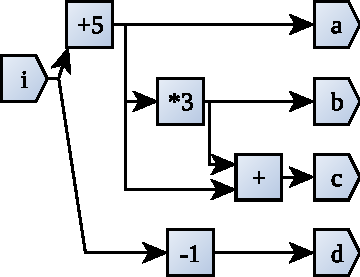
\includegraphics[width=\textwidth]{graphics/fFuncDraw.pdf}
			\end{minipage}%
			&
			\begin{minipage}[b]{0.14\linewidth}
        \begin{minted}[autogobble,tabsize=2,fontsize=\fontsize{7}{8}\selectfont]{c}
          void f(int i,
            &a,&b,&c,&d){ 
            
            
            a = i + 5;
            b = a * 3;
            
            c = a + b;
            d = i - 1;
            
          }
				\end{minted}
			\end{minipage}
			&
			\begin{minipage}[b]{0.19\textwidth}
        \begin{minted}[autogobble,tabsize=2,fontsize=\fontsize{7}{8}\selectfont]{vhdl}
        f : process(clk)
        begin 
          if rising_edge(clk)
          begin
            a <= i + 5;
            b <= a * 3;
            â <= a;--cyc dly
            c <= â + b;
            d <= i - 1;
          end; 
        end process;
				\end{minted}
			\end{minipage}
			&
			\begin{minipage}[b]{0.20\textwidth}
        \begin{minted}[autogobble,tabsize=2,fontsize=\fontsize{7}{8}\selectfont]{scala}
        def f(i : DFSInt[32])= 
        {
        
          
          val a = i + 5
          val b = a * 3
          
          val c = a + b
          val d = i - 1
          (a,b,c,d) //tuple of
        }           //four
        \end{minted}
			\end{minipage}
			\\
			\hline
		\end{tabular}
		\begin{tablenotes}
			\item [†] Some type annotations were removed for brevity.
			\item [‡] \code{â} represents a clock cycle delay of \code{a}.
		\end{tablenotes}
	\end{threeparttable}
\end{table*}%

\section{Concurrency and Data Scheduling Abstractions}
\label{sec:concurrency_abstractions}

Concurrency and data scheduling abstractions rely heavily on language semantics. In this section, we explore semantics of three distinctively different languages: C++, VHDL, and DFiant. 

Consider the function $f$ and its implementations, as detailed in Table \ref{tbl:DataSchedDefImpl}. Despite similar code appearance, the semantics are very different, as depicted in Fig. \ref{fig:DataSchedGraph}. The following subsections qualify these semantics.


\subsection{C++ Semantics}
Sequential programming models, such as C++, do not have concurrent semantics. Data scheduling order is set by \textit{code statement order}, and cannot be pipelined\footnote{We only observe language semantics. Out-of-order or multi-processor executions may still apply.}. HLS utilities extends these languages with $pragma$ directives that change semantics. We observe the C++ $f$ implementation as follows:

\begin{figure}[t]
	\centering
	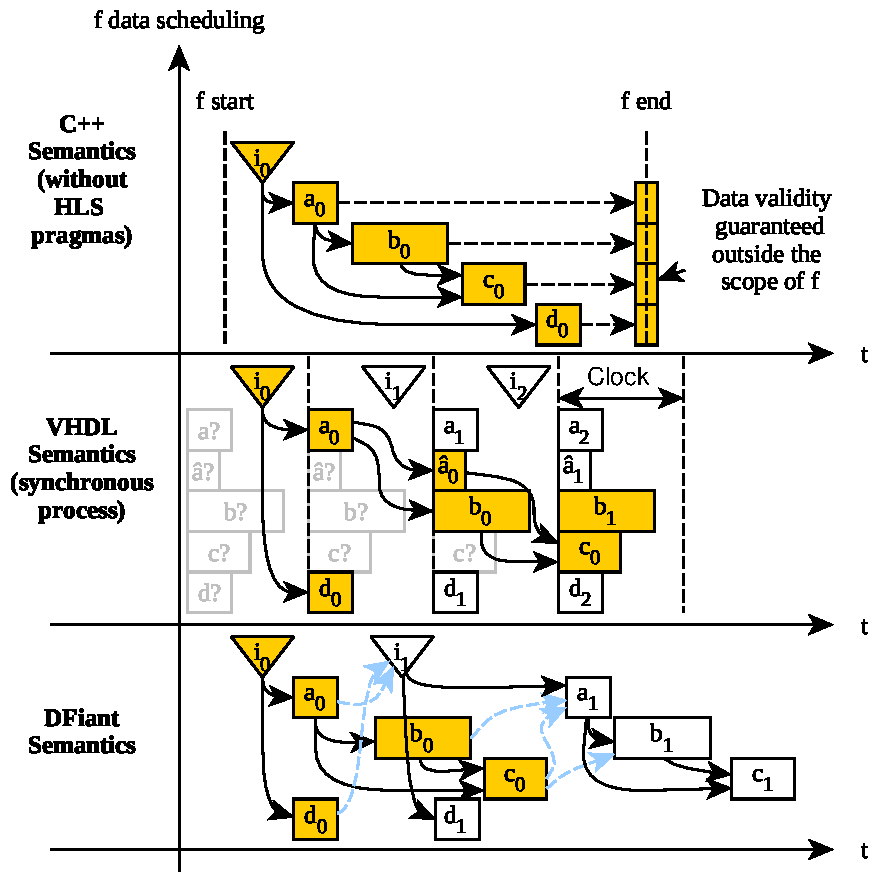
\includegraphics[width=0.6\textwidth]{graphics/DataScheduling.pdf}
	\captionof{figure}{$f$ data scheduling semantics in C++, VHDL, and DFiant}
	\label{fig:DataSchedGraph}
\end{figure}

\begin{enumerate}
	\item All statements are variable assignments.
	\item $d$ is independent of $a$, $b$, and $c$, but cannot be scheduled concurrently. Additionally, $a$ cannot be safely read until $f$ ends. Proper pragmas allow dataflow analysis and function inlining to overcome these limitations.
	\item Time between/of the data operations is unconstrained. The code does not restrict the functional requirement and will maintain correctness for every hardware synthesis fitting its semantics. 
\end{enumerate}  

\subsection{VHDL Semantics}
The RTL programming model is concurrent. Data scheduling is manual and clock-bound, while the order is set by the \textit{assignment cycle-time}. VHDL process semantics are different for \textit{signals} and \textit{variables}: signals are updated when the process ends, while variables are updated instantly. When embedded in a signal edge-detection conditional construct, both signals and variables can be interpreted as registers, depending on the context. We observe the VHDL $f$ implementation as follows:

\begin{enumerate}
	\item All statements are synchronous signal assignments with an explicit single-clock dependency. Clocked $f$ imposes time restrictions to $f$. Although this implementation does not contradict the formal definition of $f$, its correctness is guaranteed solely under these restrictions.
	\item A latency balancing register added to maintain correctness of the $c$ assignment pipeline\footnote{We can use VHDL variable to avoid latency balancing, by forming a combinational circuit.}. 
	\item Data is scheduled for every clock cycle, thus creating a pipeline. Each output signal is valid at a different time. Invalid outputs may be accessed, since VHDL has no implicit $guard$ semantics. More hardware is required to match the output cycle-latencies, and implement explicit guards.
	\item The implementation is very fragile and has limited reusability. Foremost, VHDL process construct alone is not reusable, and requires an \textit{entity-architecture} encapsulation for structural instantiation. Additionally, $f$ is tightly-coupled to $clk$ timing and logic propagation delay. The slightest change in requirements or target device can lead to a painful redesign. 
\end{enumerate}

\subsection{DFiant Semantics}
DFiant has a dataflow programming model. Data scheduling order, or \textit{token-flow}, is set by the \textit{data dependency}. Essentially, the DFiant semantics schedules all independent dataflow expressions concurrently, while dependent operations are synthesized into a guarded FIFO-styled pipeline. Dataflow branches are implicitly forked and joined. Unused nodes, semantically, always consume tokens, and are discarded during compilation. We observe the DFiant $f$ implementation as follows:

\begin{enumerate}
	\item All expressions are dataflow variable declarations.
	\item Concurrency is implicit, and $f$ is coded intuitively, in a sequential manner, since dataflow dependency is oblivious to statement order. 
	\item All scheduling is implicitly guarded by its dependencies. For example, $a$ is forked into both $b$ and $c$ operations, while $c$ joins branches from $a$ and $b$.
	It is impossible to read an invalid result or an old result (without extending semantics further).
	\item DFiant semantics are intuitive: data is consumed only when it is ready and can be accepted by all receiving nodes, while back-pressure prevents data loss. 
\end{enumerate} 


\subsection{Semantics Comparison}
Comparing DFiant and VHDL, it is evident that DFiant is less verbose and has better semantics for code reuse. The given VHDL implementation is a private case for DFiant, since it is only one of many possible solutions, while DFiant relies on its compiler to generate hardware in respect to design constraints. DFiant prevents $f$ users from reading invalid values, while in VHDL it must be programmed explicitly. Bluespec and Chisel have similar semantics to VHDL, thus suffer from related limitations (e.g., explicit pipelining). Fortunately, they both can provide guarded types that prevent invalid data use.

Comparing DFiant and C++, we observe that C++ HLS tools rely on code analysis and pragma directives to change the semantics of their sequential code, while DFiant has its own dataflow type system that guarantees its seamless concurrent semantics. Consequently, C++ HLS tools limit language constructs and hierarchies which are not supported by the analysis algorithms (e.g., recursion), in contrary to DFiant which supports all finite Scala constructs (e.g., finite generation loops and recursions). 
%We believe that constraint directives should not change semantics but refine them.

Contrarily, tandem operations are described more naturally in C++, and loops are utilized to describe repetitive dependent tasks. With proper pragmas, C++ loop iterations can run concurrently, but since they can also run sequentially, loops, and nested loops especially, may be semantically confusing. For this reason, DFiant does not support loops, same as VHDL (hardware generation loops are supported), and opts for state machine semantics to describe sequential operations. %We cover state in the next section. 
%We further compare DFiant against other HLS tools and languages in Section \ref{sec:related_work}. 


\begin{figure}[h]
	\vspace*{-3ex}
	\centering
	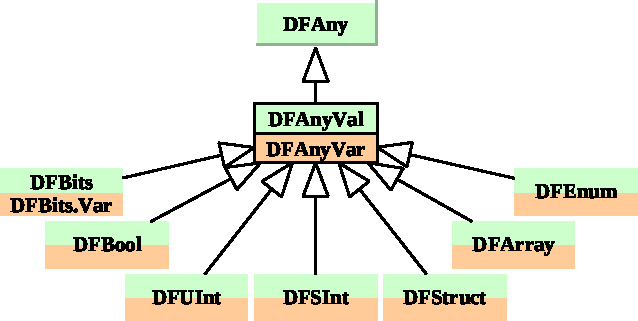
\includegraphics[scale=0.7]{graphics/Inherit.pdf} 
	\captionof{figure}{DFiant dataflow types: simplified inheritance diagram}
	\label{fig:Inherit}
\end{figure}

%\setalgorithmicfont{\small}
\begin{figure*}[h]
  \centering
  \begin{subfigure}[b]{0.5\textwidth}
    \begin{minted}[tabsize=2,gobble=3,frame=single,framesep=2pt, fontsize=\fontsize{7}{8}\selectfont]{Scala}
    class AES_DFKeySchedule(Nk: Int, Nb: Int, Nr : Int) 
      extends AES_DFWords(Nb*(Nr+1)){
      val Rcon = Array[Int](0x00000000, ...)
      def KeyExpansion(key : AES_DFKey): Unit = {
        val temp = AES_DFWord()
      
        for (i <- 0 until Nk)
          this(i) := key(i)
      
      
      
        for (i <- Nk until Nb*(Nr+1)) {
          temp := this(i-1)
          if (i % Nk == 0)
            temp := temp.RotWord().SubWord() ^ Rcon(i / Nk)
          else if ((Nk > 6) && (i % Nk == 4))
            temp := temp.SubWord()
          
          this(i) := this(i-Nk) ^ temp
        
        }
    } }
    \end{minted}
    \caption{DFiant code}
  \end{subfigure}%
%  \hfill
  \begin{subfigure}[b]{0.5\textwidth}
    \begin{minted}[tabsize=2,gobble=3,frame=single,framesep=2pt, fontsize=\fontsize{7}{8}\selectfont]{text}
    //comment line for alignment
    //comment line for alignment
    Rcon = [00000000, ...] 
    KeyExpansion(byte key[4*Nk], word w[Nb*(Nr+1)], Nk) begin
      word temp
      i = 0
      while (i < Nk)
        w[i] = word(key[4*i],key[4*i+1],key[4*i+2],key[4*i+3])
        i = i+1
      end while
      i = Nk
      while (i < Nb * (Nr+1)]
        temp = w[i-1]
        if (i mod Nk = 0)
          temp = SubWord(RotWord(temp)) xor Rcon[i/Nk]
        else if (Nk > 6 and i mod Nk = 4)
          temp = SubWord(temp)
        end if
        w[i] = w[i-Nk] xor temp
        i = i + 1
      end while
    end
    \end{minted}
    \caption{AES spec. pseudo code reference}
  \end{subfigure}
	\vspace*{-4ex}
  \caption{AES KeyExpansion code example}\label{fig:AES}
\end{figure*}

\section{The DFiant Type System}
\label{sec:type_system}
DFiant is a Scala library, hence it inherently supports type safe and rich language constructs. DFiant brings type driven development concepts to hardware design, by creating an extensible dataflow class hierarchy, with the trait \code{DFAny} at its head. 
%(similar concept to Scala's Unified Types hierarchy)
\code{DFAny} contains all properties that are common to every dataflow variable. 
%(e.g., \code{.width} represents the number of bits contained by the variable)
Fig.~\ref{fig:Inherit} illustrates a simplified inheritance diagram of DFiant's dataflow types. 

Fig.~\ref{fig:AES} depicts part of our DFiant Advanced Encryption Standard~\cite{pub2001197} (AES) cipher implementation alongside its specification pseudo code reference. The DFiant code is similar or even simpler in comparison and does not employ global functions. We compared the complete DFiant AES code to three RTL designs~\cite{das2010fully}\cite{hsing2013aes}\cite{salah2013aespipe}. DFiant provides the same functionality with 33-50\% lines of code.
Furthermore, the DFiant code is timing-agnostic and device-agnostic, thus tasking the compiler to construct the hardware fitting the target device and non-functional requirements (e.g., throughput, latency). When constrained by the appropriate target throughput, the DFiant compiler generated an RTL design that acheived better performance than the cited RTL designs.

%Since DFiant is Scala-based, the Scala IDE was utlized for debugging. It was also extremely easy to debug the code step-by-step using
%watches and console printouts. This would have been impossible to do in native HDL
%languages like VHDL and Verilog. After we fixed everything to work in software debugging backend, we have compiled the design to verilog using the hardware construction
%backend, and everything worked in RTL simulation as well.


%The DFiant type system provides the following features:
%\paragraph*{\bf \em Bit-Accurate Operations and Data Structures} 
%All DFiant's dataflow types are bit-accurate and structurally static, with their bit-width set upon construction (e.g., \code{DFBits[5]} is a 5-bit vector). Operations between dataflow variables produce a bit-accurate result with the proper type inference. For example, an addition between an unsigned 5-bit variable (\code{DFUInt[5]}) and a signed 10-bit variable (\code{DFSInt[10]}) produces an adder that can be implicitly converted to a 10-bit signed variable, if carry is not required, or an 11-bit signed variable by explicitly invoking \code{.wc} from the addition.
%
%DFiant also allows operations between dataflow types and their corresponding Scala numeric types, by treating the Scala numeric types as constants (e.g., addition between \code{DFSInt} and \code{Integer} variables). A constant in the dataflow graph is a node that can produce infinite tokens of the same value.   
%
%\paragraph*{\bf \em Mutability} 
%\label{sec:mutability}
%DFiant supports dataflow variables mutability via the \code{:=} operator. Do not confuse with Scala-level mutability which is enabled by using \code{var} instead of \code{val}. Each dataflow class has two variations: an immutable class, which inherits from \code{DFAny\textbf{Val}} and a mutable class, which inherits from \code{DFAny\textbf{Var}} and accepts \code{:=}. The difference between the types enforces an immutable right-hand-side (RHS), where required, and a mutable variable creation. Consider, for instance, the DFiant implementation of \code{g} in Table \ref{tbl:StateExDefImpl}: \code{a} is immutable because it is a RHS addition between the dataflow variable \code{i} and a literal value \code{5}. Contrarily, \code{c} is mutable, since it is a dataflow variable constructor (\code{.init} constructs a new initialized variable, while preserving the mutability trait). 
%
%Fig.~\ref{fig:Inherit} demonstrates a dual class definition for every type  (immutable and mutable). The naming convention helps to reason about the mutability. For example, \code{DFBits} and \code{DFBits.Var} are immutable and mutable classes, respectively. Constructing a new variable via \code{DFBits} (e.g, \code{val a = DFBits[5]}) returns the mutable \code{DFBits.Var[5]}. Usually, we either receive or return an immutable type, hence we do not require annotating a type with its mutable variation. In cases where we want to return a mutable type, we annotate it as an output port (see Section~\ref{sec:io_ports}).
%
%\paragraph*{\bf \em Bit Aliasing and Casting} 
%Aliasing in DFiant enables referencing a part of a dataflow variable, by invoking \code{.bits(hiIdx, loIdx)}, which creates a bits vector alias that references the original variable at the given index parameters. Every change of a dataflow variable affects its alias and vice versa (similar to VHDL's signal aliasing). Since this function also casts the variable as \code{DFBits}, this feature is used as a raw-data cast between different dataflow types. Aliasing of an alias is also possible, while maintaining relative bits indexing. Aliasing preserves the mutability trait: an alias of an immutable variable is immutable, while an alias of a mutable variable is mutable. 
%
%\paragraph*{\bf \em Structural Composition and Generation} 
%
%\begin{figure}[h]
%  \centering
%  \begin{minipage}[b][3cm][b]{0.57\linewidth}
%    \vfill
%    \begin{minted}[xleftmargin=1.5em,linenos,autogobble,tabsize=2,framesep=1pt, frame=single,fontsize=\fontsize{7}{8}\selectfont]{scala}
%      val bits128 = DFBits[128] := 0
%      val alias64 = bits128(127, 64)
%      val alias32 = alias64(31, 0)
%      val dbl = DFDouble := 1.0
%      dbl.bits(7,0) := 0x28
%      bits128(127) := 1
%      bits128(63, 0) := dbl.bits()
%      alias32(16, 8) := 0x57		    
%    \end{minted}
%    \vfill
%    \subcaption{DFiant code}
%  \end{minipage}%
%  \hfill
%  \begin{minipage}[b][3cm][b]{0.40\linewidth}
%    \centering
%    \vfill
%		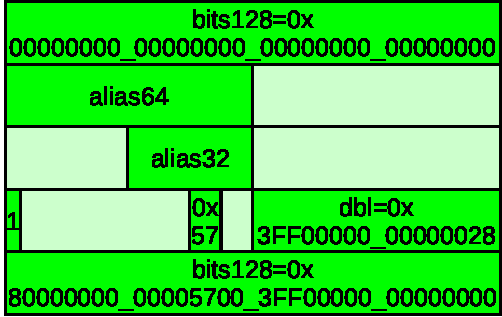
\includegraphics[width=\linewidth]{graphics/Aliasing.pdf} 
%    \vfill
%    \subcaption{Contents of \code{bits128}}
%  \end{minipage}
%  \captionof{figure}{Bit aliasing and casting example}
%  \label{fig:Aliasing}
%\end{figure}
%
%Fig.~\ref{fig:Aliasing} demonstrates aliasing code and its effect on the contents of a dataflow variable (\code{bits128}). Each line code does as follows:
%\begin{enumerate}
%  \item Constructs a new 128-bit vector, \code{bits128}, and clears all its bits.
%  \item Creates a new alias, \code{alias64}, which references the most significant 64 bits of \code{bits128}. Since \code{bits128} is a \code{DFBits} variable, there is no need to invoke \code{.bits()}, and we can apply the required indexes directly.
%  \item Creates a new alias, \code{alias32}, which references the least significant 32 bits of \code{alias64}, which reference bits 64 to 95 of \code{bits128}.
%  \item Constructs a new double precision floating point dataflow variable, \code{dbl}, and initialize its value as \code{1.0} (hexadecimal value of \code{0x3FF00...0}).
%  \item Modifies the least significant byte of \code{dbl}.
%  \item Sets the most significant bit of \code{bits128}.
%  \item Assigns \code{dbl} to the least significant 64 bits of \code{bits128} through casting. All the bits of \code{dbl} are selected because \code{.bits()} is invoked without index parameters.
%  \item Modifies a byte of \code{bits128}.
%  
%\end{enumerate}
%
%
%DFiant expands traditional structural composition capabilities by utilizing Scala's object oriented features such as inheritance and polymorphism, as well as finite loops and recursive composition. The hierarchical compositions provide the scope and dependencies for the dataflow variables. The hierarchy itself is transparent to the dataflow graph, as if the entire design is flattened, inlined, and unrolled. Therefore, hierarchies in DFiant are synthesizable, highly reusable, and do not affect the design performance (may affect compilation time). Different composition examples are available in Table~\ref{tbl:Box}.
%
%\paragraph*{\bf \em IO Ports} 
%\label{sec:io_ports}
%The class \textit{Box} from Table~\ref{tbl:Box} can also be coded as demonstrated in Fig.~\ref{fig:IOBox}. The annotation \code{DFVar $<>$ Dir} controls \textit{DFVar}'s access by encapsulating the variable with the dataflow port class, \code{DFPort}: an \code{IN} port can only be read (immutable), while an \code{OUT} port can only be modified (unreadable). DFiant has implicit conversions in place that selectively converts between \code{DFPort} and \code{DFAny} instances, without breaking mutability rules and type safety. The port annotations match the capabilities of traditional HDLs, and are noticeably absent from HLS languages such as C++. 



\section{Proof of Concept}
\label{sec:evaluation}
In this section we demonstrate DFiant frontend and backend compilers as a proof of concept the preliminary semantics of DFiant by implementing two case studies: an AES cypher, and a double precision FPMul. We compare both test cases against traditional designs, and demonstrate competing performance while simplifying code verbosity significantly. 

\subsection{Methodology}
We implemented both test cases in DFiant, constrained them by a variance of minimum frequency requirements, and compiled them to RTL. The DFiant compiler automatically pipelined the design to achieve the required minimum frequency, and generated an RTL verilog file and a TCL constraints file. For a baseline we obtained equivalent open-source RTL cores and Vivado HLS implementations, where possible. We disabled the DFiant backend support for pipelined valid/ready signaling and a blocking back-pressure, since the RTL cores did not support this capability.

We chose the following comparison metrics: the maximum clock frequency, clock cycle latency, utilizations of both look-up tables (LUTs) and flip-flop registers (FFs), and lines of code (LoC). Digital signal processing (DSP) block utilization was zero for AES and equivalent for FPMul across all designs, thus neglected from the table. a We used Xilinx Vivado to synthesize and implement the RTL design for a Virtex-7 FPGA, part number: xc7vx485tffg1761-2. The tool was configured to use default strategy for both synthesis and implementation processes. For each design, we recorded the maximum clock frequency, LUTs, and FFs. We recorded the design latency as reported by the DFiant and Vivado HLS compilers, and the RTL cores documentation. Finally, we automatically counted the LoC \cite{danial2009cloc}, applied standard score normalization (0-100) to all metrics, and assured higher values indicate better score for all metrics. Mean score of all metrics is presented as well.

\subsection{Case Study: AES Cypher}
For baseline comparison we used three AES cypher RTL designs from opencores.org: Das core \cite{das2010fully}, Hsing core \cite{hsing2013aes} and Salah core \cite{salah2013aespipe}. Additionally, we obtained a Vivado C++ HLS design~\cite{oflynn2014rapid}. All these designs are fully pipelined, meaning that in every cycle the design accepts new key and data inputs, and emits an encrypted data output, delayed by a fixed design latency.

We compiled the DFiant and Vivado HLS designs with three target clock frequencies: 200 MHz, 300 MHz, and 450 MHz. We named the designs accordingly (e.g., DFiant\_200 is the 200MHz target design). We collected the results in Table~\ref{tbl:AES_Compare_Table}, and displayed their normalized standard score in Fig.~\ref{fig:AES_Compare_Graph}. We added the supported key types quantity as a metric, since some designs support 128bit keys and do not include 192bit and 256bit keys as well. The table also includes an 'SBox BRAM Use' column, since some designs do not use memory to implement the AES SBox function.

\begin{table*}[t!]
  \centering
  \begin{minipage}[t][5cm][t]{0.62\linewidth}
    \centering
    \captionof{table}{AES Cypher RTL Designs Comparison\\(the numbering on the left associates configurations with \fig{fig:AES_Compare_Graph})}
    \label{tbl:AES_Compare_Table}
    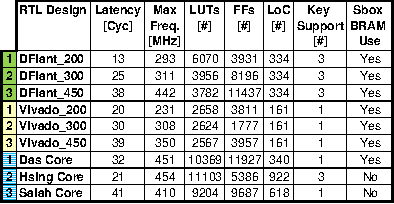
\includegraphics[scale=1]{graphics/AES_Compare_Table.pdf} 
  \end{minipage}
  \hfill
  \begin{minipage}[t][5cm][t]{0.37\linewidth}
    \centering
    \captionof{table}{FP Mult. RTL Designs Comparison\\(the numbering on the left associates configurations with \fig{fig:FP_Compare_Graph})}
    \label{tbl:FP_Compare_Table}
    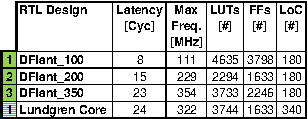
\includegraphics[scale=1]{graphics/FP_Compare_Table.pdf} 
  \end{minipage}
  \begin{minipage}[b][3.8cm][b]{0.62\linewidth}
  	\centering
    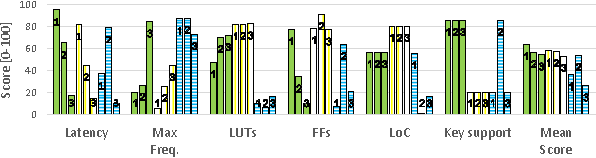
\includegraphics[height=3cm]{graphics/AES_Compare.pdf} 
    \captionof{figure}{AES cypher RTL designs score comparison (higher = better)\\ \quad}
    \label{fig:AES_Compare_Graph}
  \end{minipage}
  \hfill
  \begin{minipage}[b][3.8cm][b]{0.37\linewidth}
    \centering
    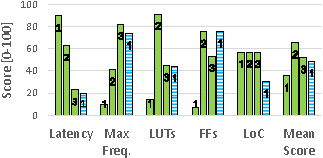
\includegraphics[height=3cm]{graphics/FP_Compare.pdf} 
    \captionof{figure}{FP multiplication RTL designs score comparison (higher = better)}
    \label{fig:FP_Compare_Graph}
  \end{minipage}
\end{table*}

The Hsing core clearly has the best performance among the different designs (but the lowest score on LUTs utilization). The primary reason it achieved this is because it uses LUTs instead of BRAMs. This enables the synthesizer to optimize the AES SBox function, and even pipeline it. DFiant uses its \code{lookupTable} library function to implement SBox, and we have yet to enable such an option for DFiant. 

Although the DFiant-generated RTL performance is not optimal, it can still  be improved without modifying the DFiant AES code, if the DFiant compiler is optimized. Moreover, this code has an adaptive pipeline, while the RTL cores pipelines are fixed. The Vivado implementation enjoys the same advantages as DFiant, and has even less LoC. However, the Vivado code does not support all possible keys and its maximum performance is far from optimum (we did not attempt to improve the HLS pragma directives).

If we assume all metrics have the same weight, the mean score places the DFiant solutions at the top. It is difficult to determine what is truly the best solution, but DFiant clearly has the best potential for further improvement without any modification to the application code.

           
\subsection{Case Study: Double Precision FPMul}

We compared our FPMul with the open IEEE-754 compatible Lundgren core \cite{lundgren2014open} (the only IEEE-754 fully compatible FPMul RTL design we had access to). Since the core is a complete floating point unit, we disabled the unnecessary parts, reducing it to only an FPMul, for a fair comparison with DFiant's code. The DFiant code was written by using the Lundgren VHDL code as a reference design. The designs are very similar in their structure, except that DFiant is considerably less verbose, and has no explicit pipeline.

We had no access to an open Vivado HLS FPMul for comparison. We could have directly invoked a \textit{double} multiplication, but an inspection of the generated RTL revealed that Vivado HLS just instantiates an RTL floating point blackbox core. DFiant can choose to use this core as well, and achieve identical performance to Vivado HLS. Furthermore, the Vivado HLS floating point implementation is not fully compatible with IEEE-754 (e.g, does not support denormalized numbers).

Similarly to the AES case study, we collected the results in Table~\ref{tbl:FP_Compare_Table}, and displayed their normalized standard score in Fig.~\ref{fig:FP_Compare_Graph}. In comparison with the Lundgren core, DFiant\_350 is better in every criteria, aside from FFs utilization. Ultimately, DFiant out-performs its reference design of FPMul, and demonstrates its ability to provide different RTL designs for design space exploration.


\chapter{Research Trajectory: Register and State Abstraction}
\label{chap:state_abstractions}
In the previous chapter, we compared implementations of a pure (stateless) function, $f$. Typical designs, however, possess a state that is implemented via clocked registers. Registers have other functional roles, such as pipelining a data path, deriving timed signals from an input clock, and synchronizing an input signal. We believe that by avoiding explicit register use, we can design without, or very little, clock dependency. 

In this trajectory, we classify various register use-cases, and present their planned DFiant functional counterpart. The classifications are divided into three main categories: \textit{synchronous technology backend}, \textit{synchronous technology interface}, and \textit{state}. For the state classification, we also explore an impure function, $g$, and compare its implementation in VHDL, C++, and DFiant (see Table~\ref{tbl:StateExDefImpl}).

%Clocked registers have various functional roles, yet all appear the same in modern HDL designs. 
%The main reason is that devices have very small number of IO ports, measurable in the hundreds, while modern designs process trillions of bps. Designs are This, of course, forces existance of state, since pure functions must receive all inputs  . Therefore, it is impossible to avoid state in a full (\textit{top}) system hardware description. 
%When HLS abstract away the clock, it is left to the code analysis to classify what variable hold state.

\section{Synchronous Technology Backend}
Registers are often forced upon the design due to a synchronous technology choice. Since they are unrelated to the functional requirement, DFiant has no constructs to express them, and relies on its compiler to implement them properly based on the functional requirements and design constraints.
We differentiate between the following backend register uses:
\subsection{Pipelining}
DFiant auto-pipelines the design by inserting registers to split long combinational paths. The amount of pipelining is determined by designer-specified constraints, such as the maximum path cycle latency, or the maximum propagation delay between registers. 

\subsection{Synchronizers}
Sampling clock domain crossing (CDC) or asynchronous signals is exposed to metastability. Synchronizers, often composed of registers, are used to mitigate its effect and bring the design to the proper reliability. Since we aspire for a clockless design frontend, we want the synchronizers to be implicit. Currently, DFiant only supports a single clock backend, and does not require synchronizers. Once we add support for multiple clock domains and external inputs, we must address these issues as well (see Section~\ref{sec:multiple_clock_domains}).

\section{Synchronous Technology Interface}
\label{sec:sync_ifc}
Functional design requirements are often accompanied by synchronous input/output (IO) timing constraints such as clocked protocol interfaces or real-time restrictions. However, these constraints only effect the interface, and are unrelated to the design core. To maximize design portability, we apply legacy constructs solely in the periphery, while keeping the design core coded in dataflow. DFiant exposes a frontend bridge across legacy RTL constructs and its dataflow types. We differentiate between the following synchronous signaling:
\subsection{External IO and Blackbox Interfaces}
External IOs that are exposed to the top design hierarchy, or blackboxes that are exposed to the internal design core, may impose synchronous protocols (e.g., data is valid one clock cycle after address is set). Additionally, information passing between dataflow and non-dataflow regions require constraints annotations which we have yet to implement (e.g., specify the expected external input throughput for dataflow analysis). 
%DFiant supports legacy RTL constructs to synchronously interface external IOs and instantiate blackboxes. 
%\section{IO/Blackbox Interfaces}
%External IO interfaces and require dedicated frontend, as indicated in Section \ref{sec:sync_ifc}. 
%We implemented a preliminary interface between DFiant and Chisel, allowing us to tap into Chisel's hardware generation and cycle accurate simulations.
\subsection{Timers}
Timers are design constructs for outputting real-time signals, or creating derivations of timed signal inputs. For example, a target device is fed by a 100MHz clock and we want to output a UART stream at 10Mbps or toggle a led at 1Hz. Instead of directly applying registers or clock generation components, we can create functional representation of their timed use-cases. Currently, DFiant supports timers with legacy RTL constructs. We intend on including functional timers, during our work on this trajectory.

\begin{table*}
  \centering
	\captionof{table}{State Semantics Example Function, $g$: Definition and Implementations}
  \label{tbl:StateExDefImpl}
	\begin{threeparttable}
    \scriptsize
		\setlength\tabcolsep{2pt}
		\begin{tabular}{|c|c|c|c|c|}
			\hline 
			\textbf{Formal Definition} & \textbf{Func. Drawing} & \textbf{C++ Impl.}\tnote{†}~\tnote{‡} & \textbf{VHDL Impl.}\tnote{‡} & \textbf{DFiant Impl.} \\ 
			\hline
			\begin{minipage}[b][3.1cm][c]{0.25\linewidth}
				{\fontsize{7}{8}\selectfont
					\begin{equation}
					\nonumber
					\begin{split}
					&g:(i_{n})_{n\in \mathbb{N}}\rightarrow (a_n,b_n,c_n)_{n\in \mathbb{N}}\\  
					&\triangleq\left\{
					\begin{aligned}
					a_k &= i_k+5 & k\geq 0\\ 
					b_k &= i_k+i_{k-1} & k>0 \\   
					b_k &= i_k+0  & k=0 \\
					c_k &= i_k+c_{k-1} & k>0  \\ 
					c_k &= i_k+0 & k=0
					\end{aligned} 
					\right.
					\end{split}
					\end{equation}
				}
			\end{minipage}
			&
			\begin{minipage}[b][3.1cm][c]{0.18\linewidth}
				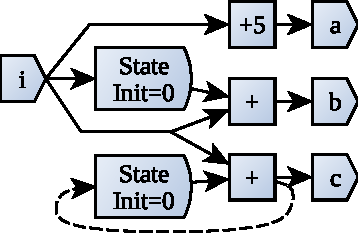
\includegraphics[width=\linewidth]{graphics/gFuncDraw.pdf}
			\end{minipage}%
			&
			\begin{minipage}[b]{0.15\linewidth}
				\begin{minted}[autogobble,tabsize=2,fontsize=\fontsize{7}{8}\selectfont]{c}
          void g(int i,
            &a,&b,&c){
           static int î=0;
           static int ĉ=0;
            
           a = i + 5;
           b = i + î;
           î = i;
           c = i + ĉ;
           ĉ = c;
          }
				\end{minted}
			\end{minipage}
			&
			\begin{minipage}[b]{0.21\linewidth}
				\begin{minted}[autogobble,tabsize=2,fontsize=\fontsize{7}{8}\selectfont]{vhdl}
          g : process(clk)
           variable î:integer:=0;
          begin
           if rising_edge(clk)
           begin
            a <= i + 5;
            b <= i + î;
            î := i;
            c <= i + c;
           end; 
          end process;
				\end{minted}
			\end{minipage}
			&
			\begin{minipage}[b]{0.24\linewidth}
				\begin{minted}[autogobble,tabsize=2,fontsize=\fontsize{7}{8}\selectfont]{scala}
          def g(i : DFSInt[32]) = 
          {
            
            
            
           val a = i + 5
           val b = i + i.prev.init(0)
           val c = DFSInt[32].init(0)
           c := i + c //prev optional
           (a,b,c) //tuple of three
          }
				\end{minted}
			\end{minipage}
			\\
			\hline
		\end{tabular}
		\begin{tablenotes}
			\item [†] Some type annotations were removed for brevity.
			\item [‡] \code{î} and \code{ĉ} represent previous state values of \code{i} and \code{c}, respectively.
		\end{tablenotes}
	\end{threeparttable}
\end{table*}%


\section{State}
State occurs when we require access to (previous) values which are no longer available on a function's inputs (e.g., cumulative sum or a state-machine's state). Table~\ref{tbl:StateExDefImpl} introduces a state function, \code{g}, and its implementation in C++, VHDL, and DFiant. The C++ implementation uses the \code{static} qualifier to preserve \code{i} and \code{c} values between \code{g} calls. Because a static variable saves its value for every call of \code{g}, the C++ implementation cannot be used in the same design more than once. The VHDL implementation invokes registers (behaviorally) to save the state. Unfortunately, registers not only save the state, but also enforce specific cycle latencies. Furthermore, both C++ and VHDL declare additional variables and place extra assignments just to save the state. DFiant overcomes all these issues and in a less cumbersome way.

The DFiant state abstraction is achievable via the \code{.prev} construct, to summon the previous dataflow variable value, and also the construct \code{.init(value)}, to create an initialized dataflow variable. The \code{:=} assignment operation is available for a mutable dataflow variable such as \code{c} (see Section~\ref{sec:mutability}). The creation of \code{c} carries within it an implicit assignment \code{c := c.prev}, which makes the next assignment of \code{c}, \code{c := i + c}, equivalent to \code{c := i + c.prev}. This is possible due to the following semantics: \textit{previous values change at the end of the DFiant code} (similarly to signal update semantics in VHDL processes). One advantage is that the code resembles its RTL counterparts, but less verbose. Another advantage is that any type of state component, like the Muller C-element\cite{muller1957theory}, can be applied with DFiant as a frontend (note that the functional drawing in Table~\ref{tbl:StateExDefImpl} has no register drawn).

%entire design or process loop semantics. DFiant variables are implicitly static.
%Functionally a register is a memory with a single write port and unlimited

We differentiate between several kinds of state: \textit{derived state},  \textit{regular state}, \textit{speculative state}, and \textit{dedicated state components}. 

\subsection{Derived State} 
A derived state is a state whose current output value is \textit{independent} of its previous value. For example, calculating output $b$ of function $g$ requires summoning previous value of $i$. 

\subsection{Regular State} 
A regular state is a state whose current output value is \textit{dependent} of its previous state value. For example, the cumulative sum output, $c$, of function $g$ is dependent on the old sum value. 

Regular and derived states differ heavily in performance improvement when the design is pipelined. A path from $i$ to $b$ can produce a token for every clock tick, and if we pipeline the addition operation to increase the maximum frequency, the maximum throughput will increase as well. Contrarily, a path from $i$ to $c$ also depends on the previous value of $c$, and if we pipeline the addition operation of that path, the extra latency may even decrease the throughput. Furthermore, $i$ is forked into several paths, and  abides by the slowest path throughput. 

\subsection{Speculative State} 
Regular state causes bottlenecks in many systems. For instance, a processor's program counter (PC) register manifests as a regular state. The processor pipeline can only be improved thanks to a speculative mechanism that predicts the next PC value to prefetch instructions (e.g., PC+4 for a branch-not-taken prediction). In case of a miss-prediction, other mechanisms take place. 

A speculative state is a regular state that can generate a new speculative value when the actual next value is not yet ready. We propose to expand DFiant's abstractions, and solve such problems functionally, by defining a speculative path, a speculation generator, a miss-prediction detector, and a miss-prediction resolution mechanism. It is our intention to describe a functional RISC-V in DFiant, and let the compiler handle the pipelining automatically.

%In some cases a regular state limits the throughput too much. For example, a program counter (PC) register for a microprocessor pipeline. If we state dependent on the PC as a regular state, it won't be possible for the pipeline to handle more than one instruction at a time. A known solution for this is to speculate on the next value of PC (good guess is branch not taken). If we guessed wrong the pipeline should ignore the prefetched instructions and restart from where the branch occurred. This allows us to generate new speculative tokens of PC, without waiting for the pipeline to supply the vi
\subsection{Dedicated State Component Abstractions}
There are several memory components available: registers, FIFOs, random access memories with one or more write/read ports, and external memory devices. Instead of aiming for a common abstraction (e.g., array), we propose building dedicated functional constructs for proper utilization of these components (e.g., providing a dual port interface for dual port RAMs).

% Such components are included in the DFiant target device library. 

%\subsection{Speculative State and a Functional RISC-V}

%\chapter{Research Trajectories}
%\label{future_research}
%Although we established its many benefits, DFiant is still missing a few milestones before it becomes a worthy HDL candidate. In the scope of this research, we plan to explore the following trajectories, in an effort to close this gap. We believe DFiant can be an invaluable tool for computer architecture research. 

\chapter{Research Trajectory: Advanced Dataflow Control}
\label{trajectory_dataflow}
So far, we demonstrated how DFiant can cover static one-to-one token transfer functions. Notwithstanding, functionality may require upsampling (e.g., duplicate each token), downsampling (e.g., drop every third token), token arrival time dependency (e.g., priority round-robin arbiter), or token value dependency (e.g., filter out odd-valued tokens). In this trajectory, we propose constructs and semantics to formulate such functions in DFiant.

\section{Static Dataflow Scheduling}
Static dataflow scheduling occurs when both input and output token rates are static and known at compile-time. Such scheduling manipulation can be supported by defining the following constructs:
\begin{itemize}
  \item \code{.next(step)} and \code{.assignNext(step)}\quad These enable referencing a future dataflow token value, potentially breaking \textit{Causality}. However, we naturally do not allow \code{x := x.next}, and protect these constructs, while internally utilizing them to create powerful public methods such as \code{Reusable}. We expect to translate all \code{next} references to state-machines using \code{prev}, during early compilation phases.
  \item \code{.split(num)}\quad Converts one dataflow variable into a sequence of dataflow elements, thereby creating a round-robin distribution between the elements. \code{num} determines the sequence size. Therefore, for a given $r$ token rate input, each output element receives a downsampled $r/num$ token rate. 
  \item \code{.merge(seq)}\quad Acts as the opposite of \code{split}. Converts a dataflow variable sequence into a single dataflow variable. Therefore, for a given $r$ token rate at each sequence element, the upsampled output token rate is $r*seq.length$. 
  \item \code{Reusable[Component]}\quad This construct enables utilizing the same component more than once, by creating an implicit state machine that schedules the tokens. Consider the example in Fig. \ref{fig:Reusable}, which has three possible implementations of a function that takes three dataflow arguments and outputs their sum. \code{sumA} invokes two \code{+} operations, thereby constructing two adders. \code{sumB} constructs two sequences on the adder's inputs and calls \code{merge}, thereby utilizing the same adder. \code{sumC} exposes how effective \code{Reusable} truly is. Not only that lines of code count is reduced, but the code is much simpler and the designer does not need to prepare ahead, according to the number of reuses adder incurs. Obviously, using a single adder instead of two reduces the output token rate by half.
  
  \begin{figure}[h]
    \centering
    \begin{minipage}{0.82\linewidth}
      \begin{minted}[autogobble,tabsize=2,framesep=1pt, frame=single,fontsize=\scriptsize]{scala}
        def sumA(a : DFUInt[32], b : DFUInt[32], c : DFUInt[32]) : DFUInt[32] = {
          a + b + c //sum using two adders
        }
        def sumB(a : DFUInt[32], b : DFUInt[32], c : DFUInt[32]) : DFUInt[32] = {
          val adder = DFUInt[32]
          val lhs = Seq(a, c)     //adder left-hand side
          val rhs = Seq(b, adder) //adder right-hand side
          adder := lhs.merge + rhs.merge //sum using a single adder
          adder
        }
        def sumC(a : DFUInt[32], b : DFUInt[32], c : DFUInt[32]) : DFUInt[32] = {
          val adder = Reusable[DFAdder[32, 32]] //Reusable adder of 32 bits vectors
          adder(adder(a, b), c) //sum using a single adder
        }
      \end{minted}
    \end{minipage}
    \captionof{figure}{\code{Reusable} construct example}
    \label{fig:Reusable}
  \end{figure}
\end{itemize}

\fig{fig:Dataflow} illustrates token flow through dataflow variables and how it influenced by \code{prev}, \code{next}, \code{split}, and \code{merge}.

\begin{figure}[t]
  \centering
  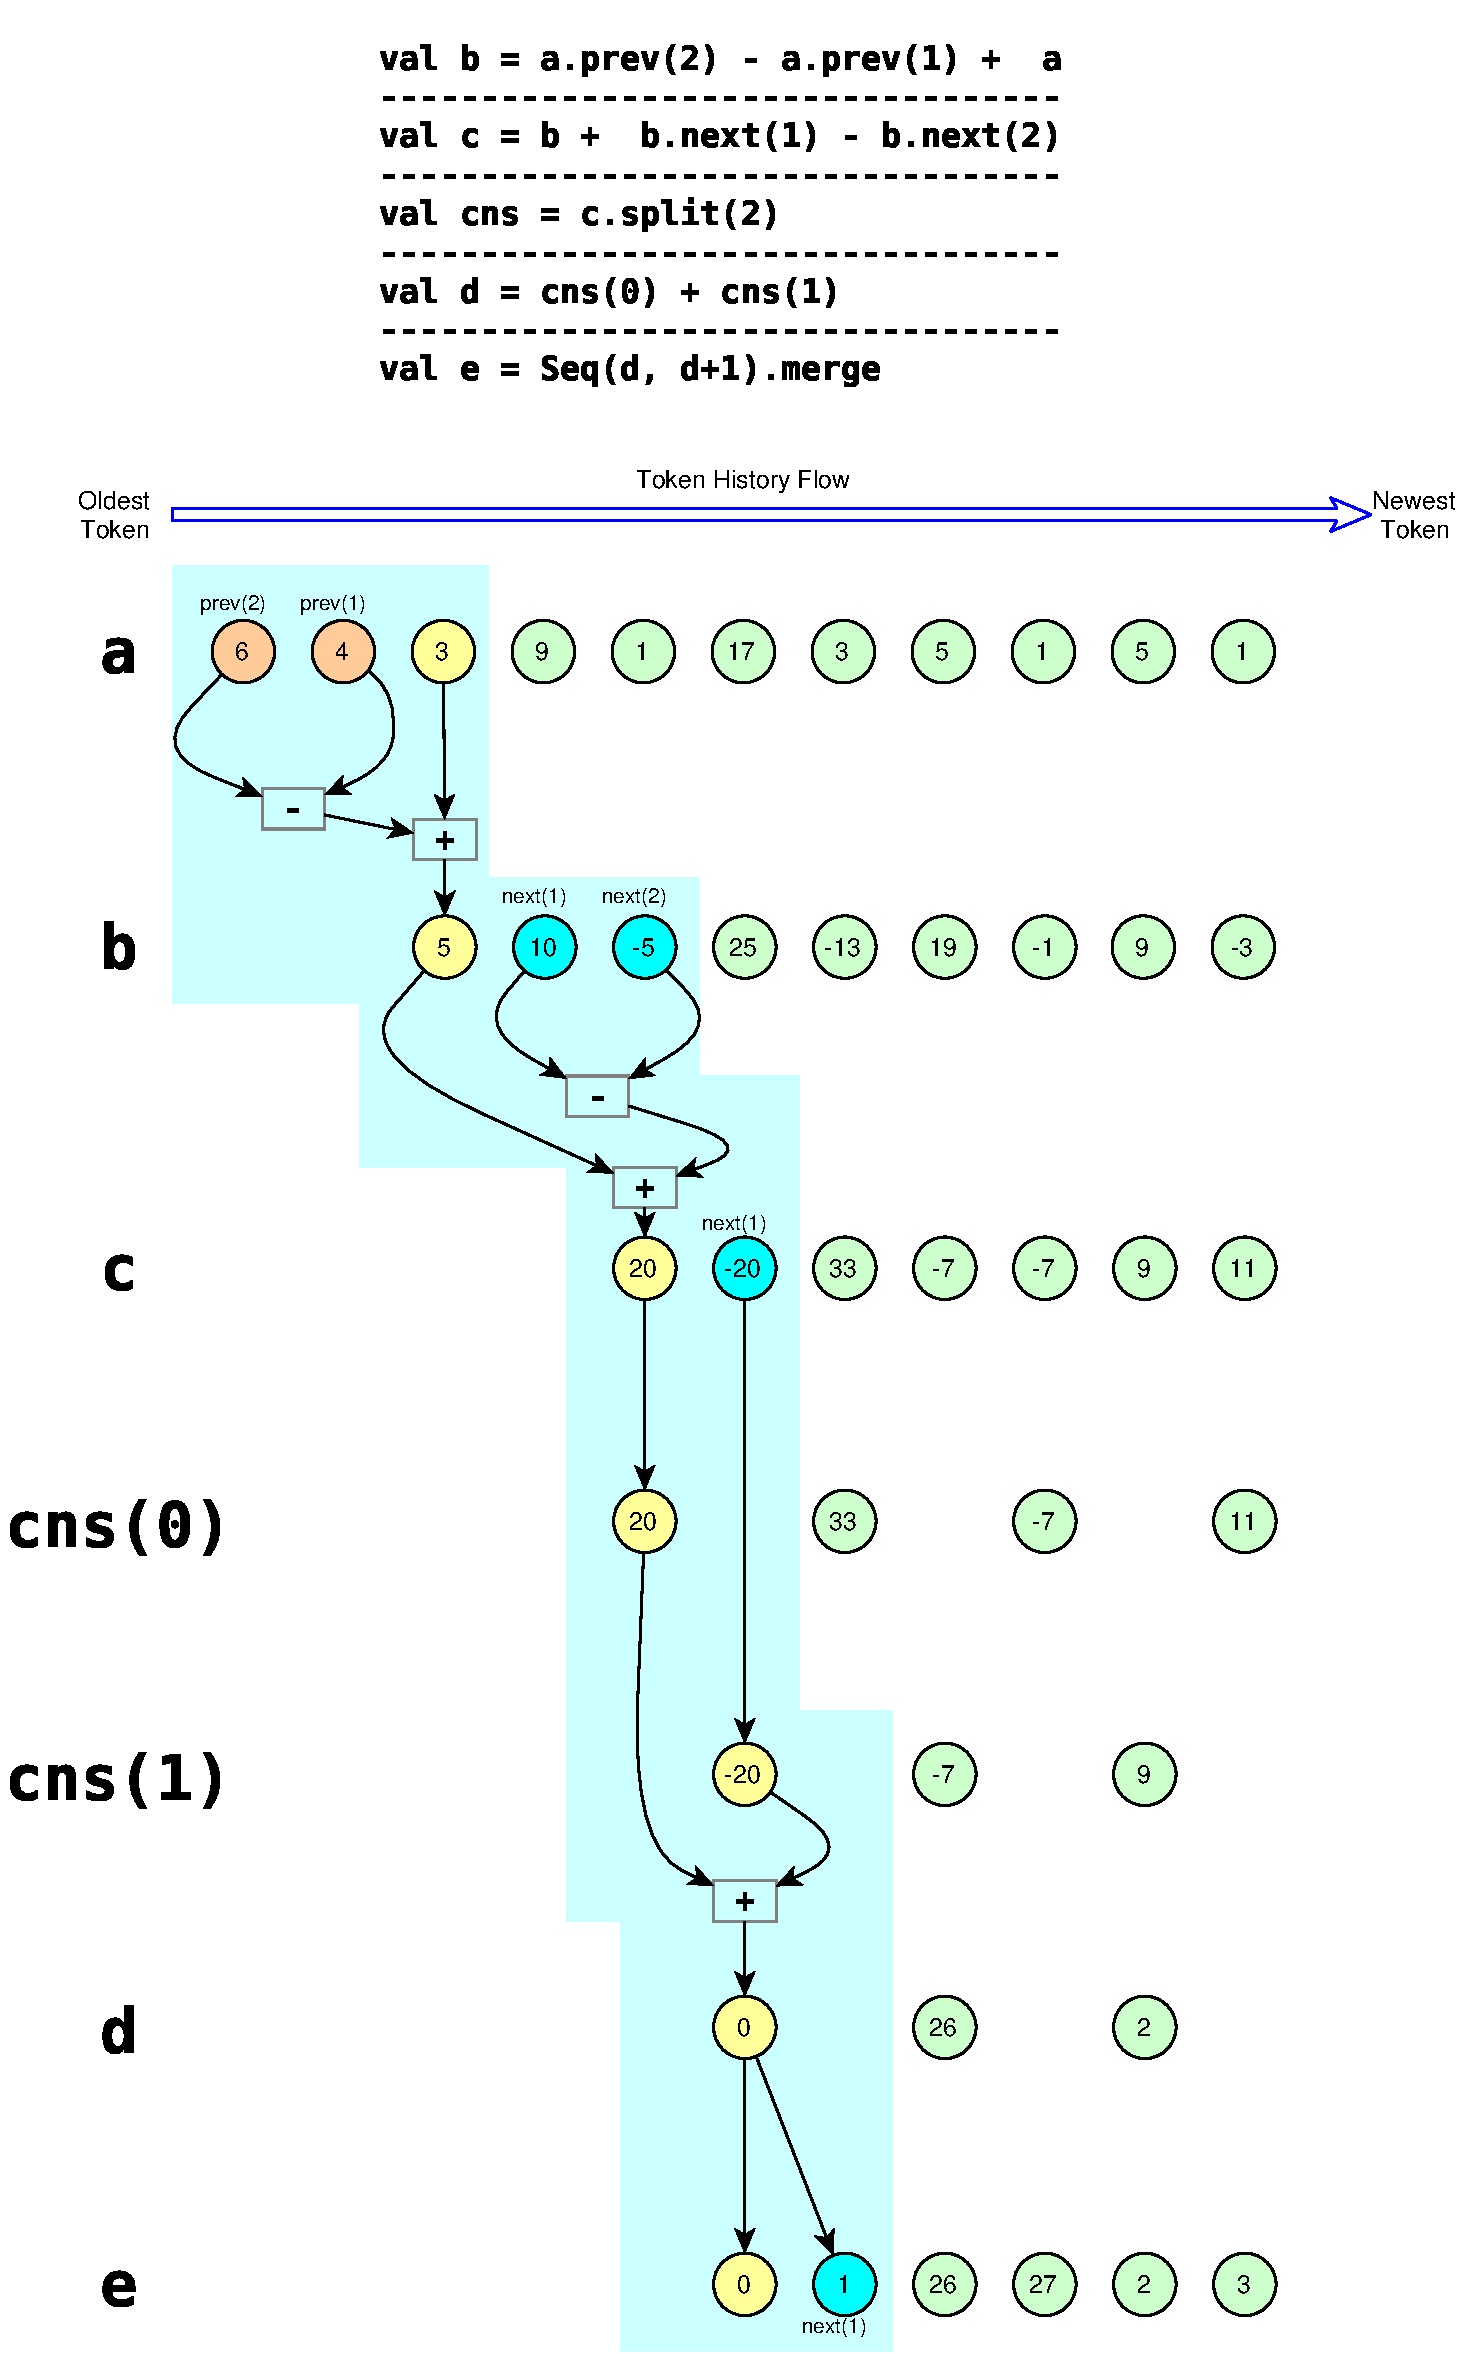
\includegraphics[width=\linewidth]{graphics/dataflow.pdf} 
  \captionof{figure}{Advanced static dataflow scheduling example}
  \label{fig:Dataflow}
\end{figure}

  
\section{Dynamic Dataflow Scheduling}
All static dataflow scheduling is \textit{blocking} and assumes a known fixed token rate. Allowing DFiant to handle dynamic dataflow scheduling, requires additional constructs to explicitly control the asynchronous FIFO-esque traits of its dataflow variables:
\begin{itemize}
  \item \code{.isNotEmpty}\quad This construct returns a boolean dataflow variable that is guaranteed to fire a single \code{true} token when the input receives a new token, but can fire an unbounded number of \code{false} tokens.
  \item \code{.dontConsume}\quad All dataflow variables are implicitly consumed in DFiant (unconnected outputs are semantically consumed as well, and are completely removed during compiler optimization). Multiple variables may consume from the same variable (dataflow fork), but if either requires to implement back-pressure, then \code{dontConsume} is used and all forked paths are delayed.
  \item \code{.isNotFull}\quad This construct returns a boolean dataflow variable that is guaranteed to fire a single \code{true} token when the output releases an old token, but can fire an unbounded number of \code{false} tokens.
  \item \code{.dontProduce}\quad All dataflow variables are implicitly produced in DFiant (to their previous value). Invoking \code{dontProduce} prevents value production. 

  \begin{figure}[H]
    \centering
    \begin{minipage}{0.49\linewidth}
      \begin{minted}[linenos,autogobble,tabsize=2,framesep=1pt, frame=single,fontsize=\scriptsize]{scala}
        def blockingMergeTwo[N](in0 : DFBits[N],
            in1 : DFBits[N]) : DFBits[N] = {
          val out = DFBits[N]
          val sel = DFBool := 0
        
          ifdf (!sel) {
            out := in0
            in1.dontConsume()
          } elsedf {
            out := in1
            in0.dontConsume()
          }
          
          
          
          
          sel := !sel
          out
        }
      \end{minted}
    \subcaption{Blocking round-robin merge example}
    \label{fig:BlockingRR}
   \end{minipage}%
   \hfill
   \begin{minipage}{0.49\linewidth}
      \begin{minted}[autogobble,tabsize=2,framesep=1pt, frame=single,fontsize=\scriptsize]{scala}
      def greedyMergeTwo[N](in0 : DFBits[N], 
          in1 : DFBits[N]) : DFBits[N] = {
        val out = DFBits[N]
        val sel = DFBool := 0
        
        ifdf (!sel && in0.isNotEmpty()) {
          out := in0
          in1.dontConsume()
        } elseifdf (sel && in1.isNotEmpty()) {
          out := in1
          in0.dontConsume()
        } elsedf {
          out.dontProduce()
          in0.dontConsume()
          in1.dontConsume()
        }
        sel := !sel
        out
      }
      \end{minted}
      \subcaption{Greedy round-robin merge example}
      \label{fig:GreedyRR}
    \end{minipage}
    \captionof{figure}{Blocking vs. Gready round-robin merge example}
    \label{fig:RRMerge}
  \end{figure}
\end{itemize}

\fig{fig:RRMerge} gives two possible round-robin \code{merge} implementations, using the dynamic control constructors. The blocking \code{merge} stops producing if either input stops producing, while the greedy \code{merge} can continue on toggling between inputs in search for new tokens to ouput.



\chapter{Research Trajectory: Design Space Exploration}
\label{chap:tarjectory_dsexplore}

DFiant is target-agnostic and can potentially compile any functional design to fit any viable target device. Nonetheless, meeting functional requirements is not enough and designers should be able to constrain the design to meet explicit performance and utilization requirements. Furthermore, operation and data scheduling, as coded by the designer, have considerable effect on the design's potential performance and utilization. In this trajectory, we propose constructs that enable designers to constrain the design, suggest scheduling alternatives, and even request an overall cost-minimized solution.
  
\section{Designer Constraints}
Constraints add non-functional information to the design. We differentiate between two types of constraints: \textit{target-specific} (e.g., IO pins), and \textit{target-agnostic} (e.g., throughput, latency, power, utilization, reliability). Design space exploration techniques typically revolve around target-agnostic constraints, but the compiler may be too limited if target-specific constraints are applied ineffectively.
Since we aim for target-agnostic designs, we propose separating and annotating constraints that bind the design to a specific target device or technology. For example, if a target device has a 200MHz input clock with a data-bus supporting up to 200 million data payloads per second, we would separate the IO constraint from the throughput requirement. The throughput requirement can be accomplished in various ways, unrelated to the target device, while the IO interface is given and fixed to specific pins. 
  

\section{Design Option Construct}
Earlier, in \fig{fig:Reusable}, we encountered three different implementations for the same functionality: $out_i=a_i+b_i+c_i$.~ The definition \code{sumA} uses two adders, while \code{sumB} and \code{sumC} only use a single adder, at the expense of throughput. Choosing either implementation affects the design's utilization and performance. \fig{fig:naiveSumOf3} provides an encapsulating definition with the boolean parameter \code{rateOpt} to select better token rate instead of better adder utilization. We can easily select the proper implementation if the design has a few \code{sumOf3} instances, but a design can have hundreds of such instances. Furthermore, if an IP component internally has \code{sumOf3} instances, it is unreasonable to propagate all the IP's \code{rateOpt} parameters to the IP's interface, first for brevity, and second to prevent implementation leaks from a functional blackbox.

  \begin{figure}[h]
	\centering
	\begin{minipage}{\linewidth}
		\begin{minted}[autogobble,tabsize=2,framesep=1pt, frame=single,fontsize=\scriptsize]{scala}
		def naiveSumOf3(rateOpt:Boolean)(a : DFUInt[32], b : DFUInt[32], c : DFUInt[32]) : DFUInt[32]= {
			if (rateOpt) sumA(a, b, c) else sumC(a, b, c)
		}
		\end{minted}
	\end{minipage}
	\captionof{figure}{Naive sum-of-three example}
	\label{fig:naiveSumOf3}
\end{figure}

To resolve this issue, we require the designer's dilemma (e.g, what to set for \code{rateOpt}) to be solved by the DFiant compiler. For this purpose, we propose new constructs: \code{designOption} and \code{designSelect}. In \fig{fig:smartSumOf3} we declare two design-options and select between them as output.
  \begin{figure}[h]
	\centering
	\begin{minipage}{\linewidth}
		\begin{minted}[autogobble,tabsize=2,framesep=1pt, frame=single,fontsize=\scriptsize]{scala}
		def smartSumOf3(a : DFUInt[32], b : DFUInt[32], c : DFUInt[32]) : DFUInt[32]= {
		  val do1 = designOption {sumA(a, b, c)}
		  val do2 = designOption {sumC(a, b, c)}
			designSelect(do1, do2) //This is an exclusive selection
		}
		\end{minted}
	\end{minipage}
	\captionof{figure}{Sum-of-three example using design option constructs}
	\label{fig:smartSumOf3}
\end{figure}

The DFiant compiler can estimate the utilization and performance from the implementation and choose the appropriate instance based on the design's global constraints. These constructs give designers similar abilities to pragma statements in Vivado HLS, but with much greater programming control (these are not pragmas, but classes within the DFiant library that can be expanded and fully-interacted with).

We are faced with a challenging algorithmic problem. A design in DFiant can have canonized design options, which may explode compilation time if we do not apply a good algorithm to select the appropriate instances. 

%We can see the the advantage to traditional HLS. The scheduling in DFiant is explicit, but DFiant also can implement mechanisms to choose a good implementation as hinted by the developer.

\section{Design to Cost}
For developers using FPGAs, a typical project starts with a specific target device in mind, which was selected based on the target application utilization estimation. The printed circuit board and logic design are then both tailored for the chosen device. An underestimation of the target application's utilization may prevent the project from completing. To counter this, an overestimation may occur, rendering a more costly product. Additionally, since different vendor devices carry a variance in production cost and power consumption, it may be crucial to select a more costly device that can save money in power requirements. 

DFiant can provide an interesting solution to these issues. Since designs can truly be device-agnostic, we can use the constraints solver to find the least costly solution from a range of potential devices for the given functional requirement. The solver can take into consideration power consumption estimation, device production cost, and other constraints.
\chapter{Research Trajectory: Alternative Backends}
\label{chap:trajectory_backend}
Currently, DFiant designs are compiled solely into a single-clocked synchronous Xilinx FPGA. The limitation is not in the language, but in the preliminary backend implementation. In this trajectory, we implement different backend possibilities to truly prove the language's agnosticity, as well as exploring advantages of asynchronous logic design, multiple clock domains, and ASIC devices. Using the same design and comparing across such backend variance may prove to be an invaluable and unique tool trait.

\section{Multiple Clock Domains}
\label{sec:multiple_clock_domains}
Implementing multiple clock domains can save power, but for modern design flow it requires different synchronous RTL description (using another clock for some processes), explicit clock generators, different constraints, and possibly CDC snchronizers. The DFiant compiler backend can generate a muli-clocked RTL design without designer hassle. It is an open question how to properly select regions for optimal clock domains.

\section{Asynchronous Logic}
As we covered in the related work chapter, asynchronous logic design has been long possible, but infrequently applied. Since DFiant is essentially asynchronous at its core, it can also utilize the proper primitives to generate an asynchronous design, while comparing it against an equivalent synchronous design.

\section{ASIC Devices}
While FPGAs have specific structure, hard-IPs, and clock-trees, ASIC design is less constrained, but creates a different set of challenges we have yet faced.

%\chapter{Other Notable Research Topics}
\label{chap:future_research}

The following topics will not be pursued in the scope of this research, but are interesting trajectories that others may pursue in a conjoint research effort:
\begin{enumerate}
	\item \textbf{Language formulation and proofs}\quad 
	\item \textbf{Partial reconfiguration}\quad 
	\item \textbf{Hardware partitioning}\quad 
	\item \textbf{Memristors logic programming}\quad 
	\item \textbf{GPGPU programming}\quad 
	\item \textbf{Approximate computing programming}\quad 
	\item \textbf{General-purpose heterogeneous platform programming}\quad 
\end{enumerate}

%
% Add any appendices here; they must come _before_ the bibliography
%
\appendix

%%%%%%%%%%%%%%%%%%%%%%%%%%%%%%%%%%%%%%%%%%%%%%%%%%%%%%%%%%%%%%%%%%%%%%%%
% References
%%%%%%%%%%%%%%%%%%%%%%%%%%%%%%%%%%%%%%%%%%%%%%%%%%%%%%%%%%%%%%%%%%%%%%%%
%\bibliographystyle{abbrv}
%\small
\onecolumn
\bibliographystyle{misc/iitthesis}
\bibliography{bib/macros,bib/references}
%\nocite{*}
%%%%%%%%%%%%%%%%%%%%%%%%%%%%%%%%%%%%%%%%%%%%%%%%%%%%%%%%%%%%%%%%%%%%%%%%

%\afterpage{\blankpage}
%\afterpage{\blankpage}
%\includepdf[pages=last-1]{heb/thesis_heb.pdf}
%\includepdf[pages=last-1]{heb/thesis_heb_first.pdf}
%\noappendicestocpagenum
%\addappheadtotoc
%
\chapter{Some sort of an appendix}
\label{appendix:somesort}

You may want to include appendices of your own volition. Also, if you've developed any computer software, that needs to go in as an appendix as well.

\section{A section}

Some appendix content here. And something nice to finish things off:




% Back Matter
% ------------

% The following command will typeset the bibliography,
% then typeset the Hebrew part of the thesis:
% - Cover page
% - Title page
% - Acknowledgements page
%  (NO table of contents or list of figures in Hebrew)
% - (Extended) abstract (1000-2000 words)
%
% based on information you've provided in the thesis-fields file
% (including the relative paths to your bib files). The Hebrew
% content will be typeset in _reverse_page_order_, i.e. first
% in the file will be the last page of the abstract, and the
% Hebrew cover page will be the last page of the file.
%
%\makebackmatter

% The resulting PDF can be printed and taken straight to binding,
% i.e. you do not need to flip any pages anywhere. Of course,
% mind the LaTeX error and warning messages, overfull hboxes etc.

\end{document}

